\documentclass[a4paper, twopage]{scrreprt}

\usepackage[ngerman]{babel}
\usepackage[utf8]{inputenc}
\usepackage[backend=bibtex, style=numeric]{biblatex}
\usepackage{hyperref}
\usepackage{graphicx}
\usepackage{url}
\usepackage{caption}

\author{Samuel Hammer}
\title{Vorgehensmodelle zur Projektentwicklung}
\subtitle{Ausarbeitung für die mündl. PRE Matura 2015}

\bibliography{quellen.bib}

\begin{document}

\maketitle
\tableofcontents

\chapter{Einleitung}
\label{ch:einleitung}
IT-Projekte können je nach konkretem Anwendungsfall unterschiedlich groß bzw. komplex werden. Um unabhängig von diesen Faktoren die Übersichtlichkeit, Organisation und Struktur eines Projektes zu gewährleisten, gibt es verschiedene Vorgehensmodelle. \newline
Die existierenden Vorgehensmodelle lassen sich grob in zwei Kategorien unterteilen: 
\begin{itemize}
	\item Klassische Phasenmodelle
	\item Vorgehensmodelle zur agilen Softwareentwicklung
\end{itemize}
Abhängig vom Anwendungsfall, können verscheidene Vorgehensmodelle verschiedene Vor- und Nachteile für das Projekt haben. In der Praxis gibt es also in den seltensten Fällen ein Modell, das für die Durchführung des Projektes hundertprozentig passt.
\begin{figure}[h]
\centering
	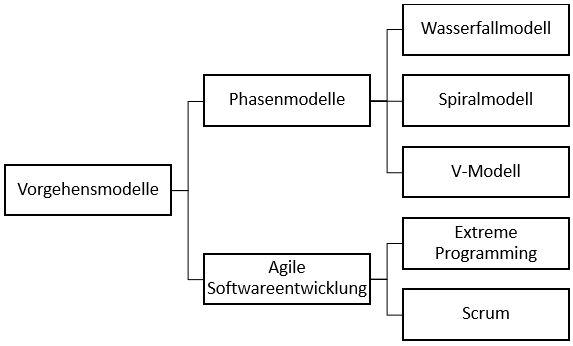
\includegraphics[scale=0.6]{Images/vorgehensmodelle_diagramm}
	\caption{Übersicht über Vorgehensmodelle\label{fig:vorgehensmodelle_diagramm}}
\end{figure}

\newpage

\section{Phasenmodelle}
\label{sec:phasenmodelle}
Phasenmodelle sind "standardisierte Projektstruckturen für die Erstellung des Projektprodukts". \footnote{\cite{wikipedia:projektphase}}
Da allerdings nicht auf jedes Projekt die selben Phasen zutreffen, gibt es verschieden Abwandlungen. Für Softwareprojekte wird in der Regel folgende Phasenstruktur verwendet:
\begin{enumerate}
	\item Anforderungen
	\item Analyse
	\item Design
	\item Entwicklung
	\item Test
\end{enumerate}
Wenn diese verschiedenen Phasen des Projektes komplett sequentiell und unabhängig voneinander stattfinden, so spricht man vom klassischen Wasserfallmodell. (Siehe Kapitel \ref{ch:wasserfallmodell}
In der Praxis hat sich das strikte vorgehen von oben nach unten (also wie ein Wasserfall) allerdings nicht bewährt, da dieses Modell es nicht erlaubt einzelne Phasen zu wiederholen.
Für diesen Fall wurden iterative Modelle entwickelt. Hier können dann einzelne Phasen wiederholt werden falls sich beispielsweise während des Projektes die Anforderungen verändern.
\section{Agile Softwareentwicklung}
\label{sec:agile_softwareentwicklung}
Agile Softwareentwicklung gibt es seit den frühen 1990er Jahren. Mit steigender komplexität der Softwareprojekte, wurde auch der Aufwand in Bezug auf das Projektmanagement immer größer. Da klassische Phasenmodelle aufgrund ihrer geringen Flexibilität nicht mehr praktikabel waren, wurde das sogenannte "Agile Manifest" verfasst. Das Agile Manifest ist ein Werk, in dem Agile Werte definiert werden, um Softwareprojekte einfacher und besser zu gestalten. Ein Auszug aus dem Agilen Manifest besagt: \paragraph*{}
"Wir erschließen bessere Wege, Software zu entwickeln, indem wir es selbst tun und anderen dabei helfen. Durch diese Tätigkeit haben wir diese Werte zu schätzen gelernt:
\begin{itemize}
	\item \textbf{Menschen und Interaktionen} mehr als Prozesse und Werkzeuge
	\item \textbf{Funktionierende Software} mehr als umfassende Dokumentation
	\item \textbf{Zusammenarbeit mit dem Kunden} mehr als Vertragsverhandlung
	\item \textbf{Reagieren auf Veränderung} mehr als das Befolgen eines Plans
\end{itemize}
Das heißt, obwohl wir die Werte auf der rechten Seite wichtig finden, schätzen wir die Werte auf der linken Seite höher ein.“ \footnote{\cite{agilemanifesto}}

\chapter{Wasserfallmodell}
\label{ch:wasserfallmodell}
Das Wasserfallmodell ist eines der ältesten linearen Vorgehensmodellen. Es ist nicht iterativ, d.h. wenn man nach dem Wasserfallmodell vorgeht, ist es prinzipiell nicht möglich einzelne Projektphasen zu wiederholen. Ursprünglich stammt das Wasserfallmodell aus der Bau- und Produktionsbranche. In anbetracht der Tatsache, dass zum damaligen Zeitpunkt noch kein eigenes brauchbares Modell zur Softwareentwicklung existierte, wurde das Wasserfallmodell schlicht und einfach für IT-Projekte adaptiert.
\paragraph*{}
Bei diesem Modell muss erst jede Phase abgeschlossen werden, bevor zur nächsten übergegangen werden kann. Daraus resultiert eine starke Unflexibilität, was das Wasserfallmodell vor allem bei Softwareprojekten sehr umständlich und beinahe unbrauchbar macht. Wenn beispielsweise in einem Projekt bereits mit der Programmierung begonnen wurde und der Kunde im Nachhinein eine Änderung an der Spezifikation vornehemen möchte, ist dies laut Wasserfallmodell nicht mehr möglich.
\begin{figure}[h]
\centering
	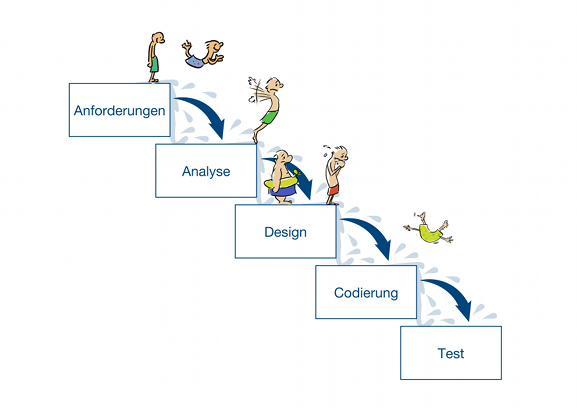
\includegraphics[scale=0.6]{Images/wasserfallmodell}
	\caption{Das Wasserfallmodell\cite{scrumkompakt:wasserfallmodell}}
	\label{fig:wasserfallmodell}
\end{figure}
Vor allem bei langläufigen Projekten ist der Einsatz des Wasserfallmodells sehr problematisch, da sich über lange Zeiträume oft die technischen Gegebenheiten und Umgebungsbedingungen ändern können. Sollte bei weit fortgeschrittenem Projektverlauf ein Fehler in einer früheren Phase entdeckt werden, ist nicht selten ein Projektabbruch die einzige Möglichkeit den Schaden einigermaßen zu begrenzen.
\paragraph*{}
Um die oben genannten Probleme aus der Welt zu schaffen, oder zumindest zu verbessern wurde das Erweiterte Wasserfallmodell nach Royce entwickelt.
\begin{figure}[h]
\centering
	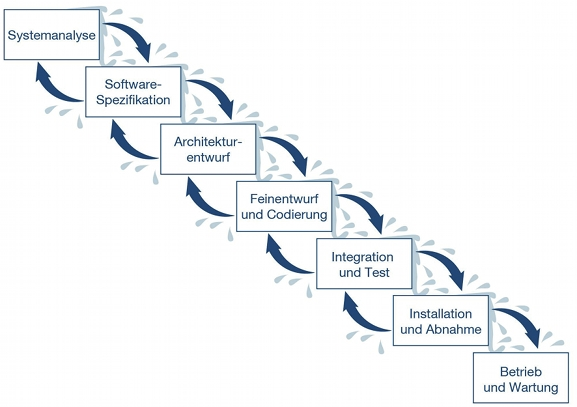
\includegraphics[scale=0.6]{Images/wasserfallmodell_erweitert}
	\caption[Erweitertes Wasserfallmodell]{Das Erweiterte Wasserfallmodell nach Royce\cite{scrumkompakt:wasserfallmodell}}
	\label{fig:wasserfallmodell_erweitert}
\end{figure}
Bei dieser Version des Wasserfallmodells sind Rücksprünge erlaubt. Nichtsdestotzotz müssen nach einem Rücksprung auf eine vorhergehende Phase, alle danach folgenden Phasen wiederholt werden. Diese Änderung verbessert das Modell zwar drastisch, allerdings werden dadurch noch lange nicht alle grundlegenden Fehler ausgemerzt.
\section{Vorteile des Wasserfallmodells}
\label{sec:wasserfallmodell_vorteile}
Da das Wasserfallmodell ein sehr altes und rudimentäres Vorgehensmodell ist, hat es, auf heutige Projekte bezogen, nicht viele Vorteile. \newline 
Ein entscheidender Vorteil ist allerdings die Einfachheit des Modells. Es lässt sich in der Praxis sehr leicht auf ein Projekt anwenden und vermittelt schnell und einfach den Eindruck von Übersicht und Kontrolle. Entgegen aller Kritik, kann das Wasserfallmodell also durchaus sinnvoll sein, solange sich das Projekt im sehr kleinen Rahmen bewegt.
\section{Nachteile des Wasserfallmodells}
\label{sec:wasserfallmodell_nachteile}
Wie bereits in Kapitel \ref{ch:wasserfallmodell} ausführlich erklärt, ist das Wasserfallmodell aufgrund der fehlenden flexibilität und der Tatsache, dass der gesamte Projektverlauf linear sein muss, in der Praxis für heutige Projekte nahezu unbrauchbar. Werden Fehler erst spät im Projektverlauf entdeckt, führt das zu sehr kostspieligen Änderungen. Des weiteren tritt durch die lange Laufzeit eines solchen Projektes, der soginannte "Return On Investment"\footnotemark erst sehr spät nach Beginn des Projektes ein.
\footnotetext{"Der Begriff Return on Investment (...) ist eine betriebswirtschaftliche Kennzahl zur Messung der Rendite einer unternehmerischen Tätigkeit, gemessen am Gewinn im Verhältnis zum eingesetzten Kapital."\cite{wikipedia:roi}}
\paragraph*{}
Auch ist es beim Wasserfallmodell oft schwierig, die einzelnen Phasen voneinander abzugrenzen. Übergänge die in der Theorie klar definiert sind, können in der Praxis oftmals eher fließend sein.

\chapter{Inkrementalmodell}

\chapter{Evolutionsmodelle}

\section{Rapid Prototyping}

\chapter{Spiralmodell}


\nocite{*}
\printbibliography

\listoffigures

\end{document}